% Исследовательская часть
\section{Описание исследования}

\hspace{1.25cm}
Были проведены замеры времени для получения максимального, минимального, среднего и медианного времён нахождения в очередях 2 и 3 и обработки на трёх стадиях (см листинг~\ref{lst:research} и график~\ref{fig:img_graph}).

\vspace{0.25cm}
\begin{lstlisting}[caption=Результаты замеров времени на разном количестве потоков, label=lst:research]
Device 1
tmin = 0.165504 ms, tmax = 0.413699 ms, tavg = 0.214917 ms, tmed = 0.211162 ms

Device 2
tmin = 0.001872 ms, tmax = 0.022422 ms, tavg = 0.007080 ms, tmed = 0.006392 ms

Device 3
tmin = 7.072097 ms, tmax = 58.647235 ms, tavg = 23.602610 ms, tmed = 22.469280 ms

Queue 2
tmin = 0.002048 ms, tmax = 0.084550 ms, tavg = 0.007184 ms, tmed = 0.003553 ms

Queue 3
tmin = 124.725575 ms, tmax = 2680.544291 ms, tavg = 1456.930559 ms, tmed = 1466.566185 ms
\end{lstlisting}

\vspace{-0.25cm}
\begin{figure}[H]
    \centering
    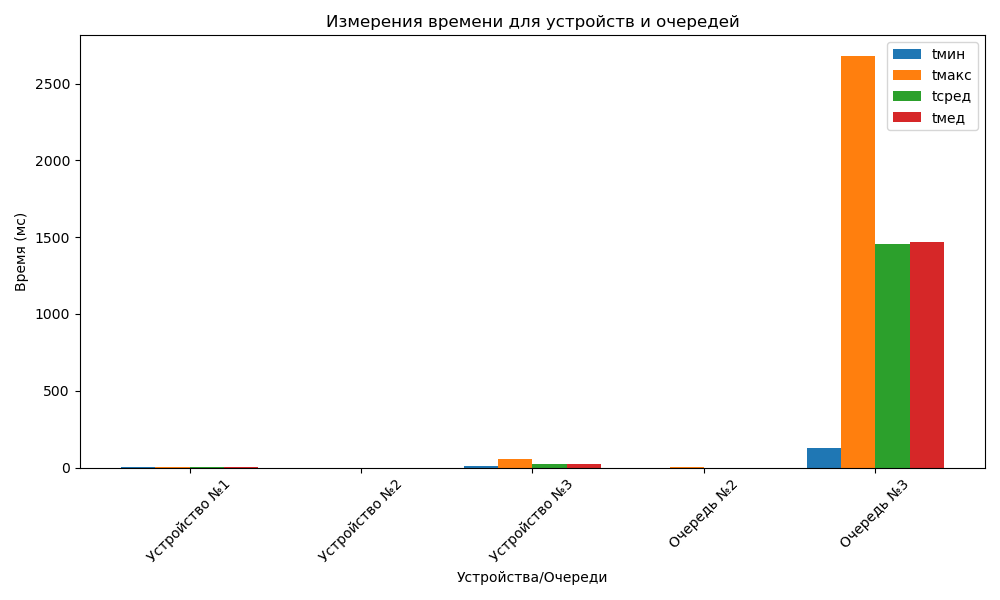
\includegraphics[width=\linewidth]{img/graph.png}
    \caption{График замеров времени для устройств и очередей}
    \label{fig:img_graph}
\end{figure}

\subsection*{Выводы}

\hspace{1.25cm}
Процесс обработки данных через потоки на первых двух стадиях (чтение данных из файла и извлечение необходимого подмножества данных) происходит достаточно быстро, с минимальными задержками. Однако на третьей стадии, связанной с записью извлечённых данных в хранилище (в данном случае в базу данных), возникает значительное замедление. Это объясняется тем, что операция записи в базу данных требует существенно большего времени по сравнению с операциями чтения и обработки данных на предыдущих этапах. Как следствие, время нахождения данных в очереди 3 превышает время, затраченное на их обработку в очереди 2, что приводит к задержкам на последней стадии обработки.
